% ----------------------------------------------------------
% Fundamentação Teórica
% ----------------------------------------------------------
\chapter{Fundamentação Teórica}\label{cap:fundamentacao-teorica}
% ----------------------------------------------------------
Nesta seção apresentam-se conceitos, fundamentos e teorias que dão suporte ao presente trabalho. Dentre eles, Computação em Nuvem, Balanceamento de Cargas e Redes Neurais Artificiais.
% ---
\section{Computação em Nuvem}\label{sec:cloud-comp}
% ---
Computação em Nuvem ou \textit{Cloud Computing} refere-se tanto à aplicações entregues como serviços via Internet quanto ao \textit{hardware} e sistemas de \textit{software} em \textit{data centers} que provém tais serviços \cite{Armbrust:2010}. Atualmente, serviços em nuvem tem criado novas oportunidades por oferecerem serviços a valores mais acessíveis para empresas de diversos tamanhos. Nos últimos anos, os benefícios econômicos tem se tornado evidentes tanto pela aceitação deste conceito, quanto pela adesão das empresas ao modelo de Computação em Nuvem \cite{raza2015}.

A Computação em Nuvem pode ser definida como um “modelo que permite acesso a rede de forma ubíqua, conveniente, \textit{on-demand} para compartilhar um grupo de recursos computacionais configuráveis (como por exemplo rede, servidores, armazenamento, aplicações e serviços) que podem ser rapidamente fornecidos e gerados com mínimo esforço de gerenciamento ou interação com o provedor”\cite{mell2011nist}. Ainda segundo Mell (2011), para ser considerado um modelo em nuvem, uma plataforma de Computação em Nuvem deve atender as características essenciais, a saber: 
\begin{alineas}
	\item \textit{On-demand self-service}, definido como a capacidade do usuário de autorregular características como armazenamento de acordo com sua necessidade e de forma automática;
	\item \textit{Broad network access}, que define a disponibilidade de acesso através da rede utilizando dispositivos diversos; 
	\item \textit{Resource pooling}, fornecimento dos serviços a múltiplos usuários, associando dinamicamente recursos heterogêneos de acordo com a demanda solicitada. Há ainda um senso de independência, visto que o usuário geralmente não possui conhecimento ou controle sobre a localização física do recurso, devido ao alto nível de abstração; 
	\item \textit{Rapid elasticity}, referente a capacidades relacionadas a elasticidade de fornecimento e alocação, em alguns casos automática, para garantir escalabilidade, dando a impressão de um serviço com capacidades ilimitadas; 
	\item \textit{Measured service}, referente ao controle e otimização automática de recursos usados aproveitando a capacidade de medição no nível de abstração apropriado para o tipo de serviço (como por exemplo armazenamento, processamento, largura de banda e número de usuários ativos). Recursos podem ser monitorados e controlados, o que garante a transparência tanto para o fornecedor do serviço quanto para o consumidor. 		
\end{alineas}

\subsection{Modelos de Computação em Nuvem e Tipos}\label{sec:mod}

Além das características essenciais, há também a separação por tipos de serviço. Neste caso, o tipo de serviço em nuvem é dividido com base em como funciona o fornecimento do serviço, bem como qual o nível de abstração atendido por aquele serviço, tal como apresentado na Figura 1. Neste sentido, há três tipos de separação: 

\begin{figure}[htb]
	\caption{\label{fig:cloud_en}Modelos de Computação em Nuvem}
	\begin{center}
		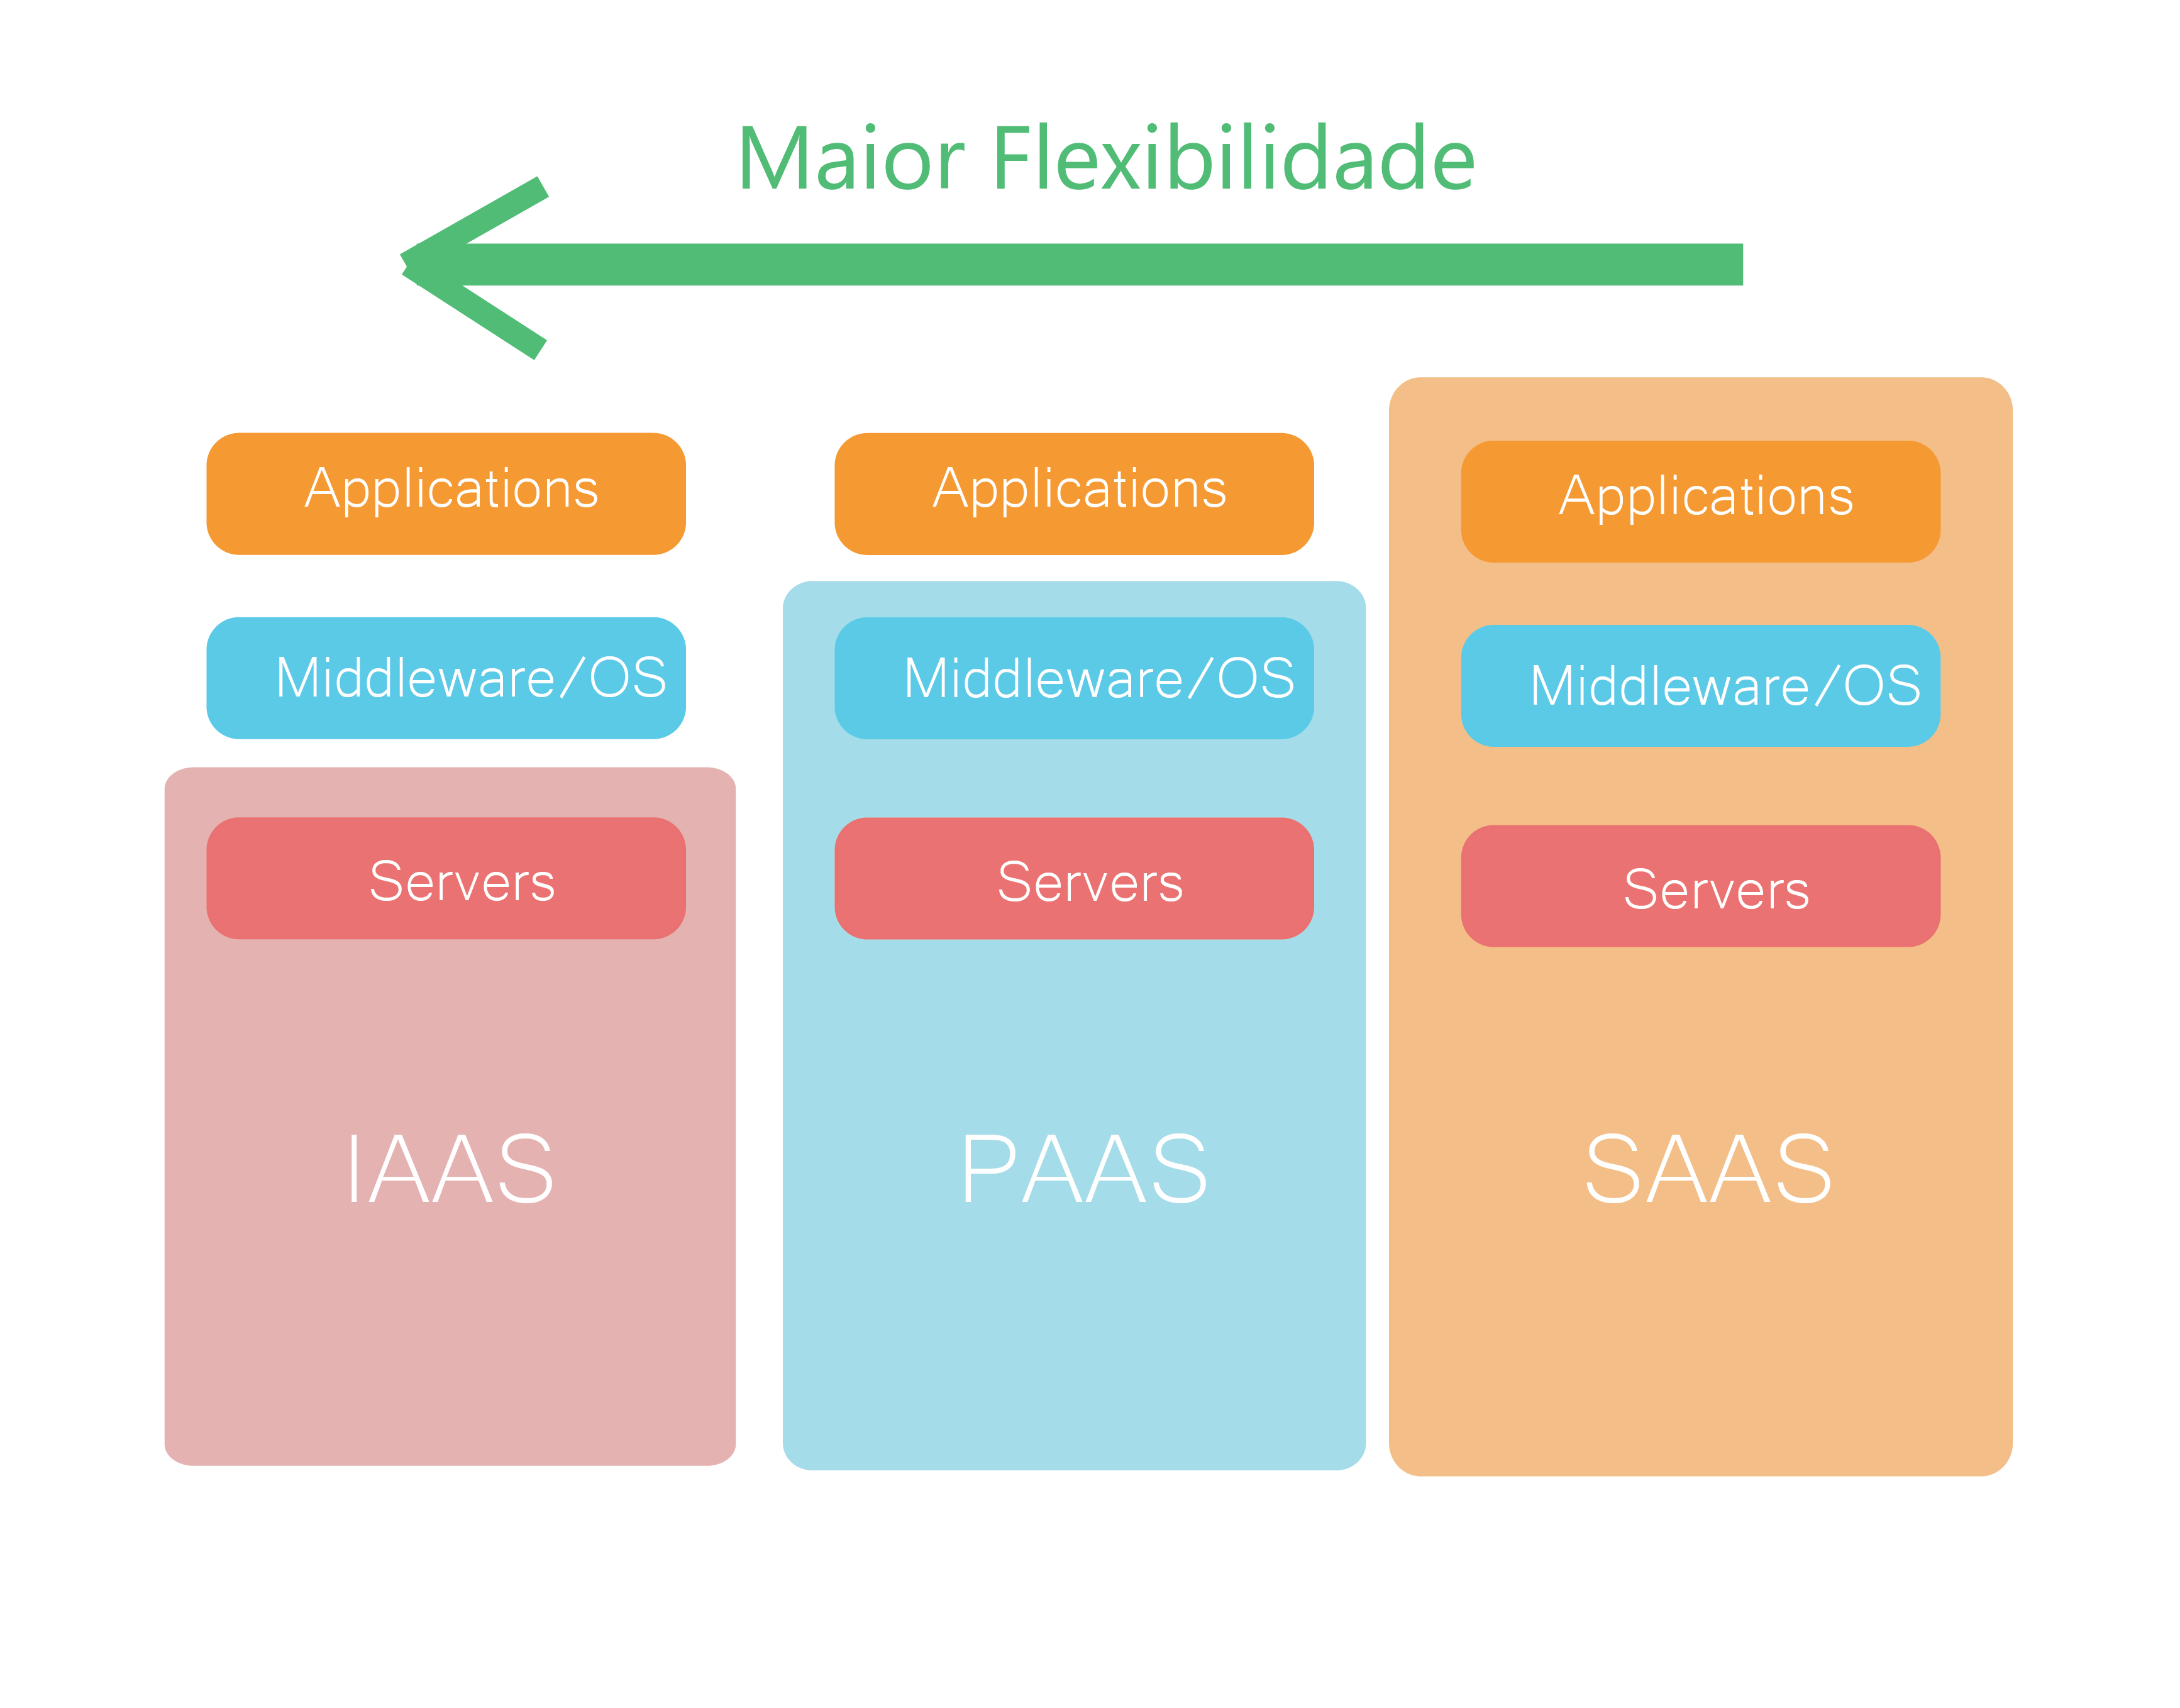
\includegraphics[width=0.50\textwidth]{img/cloud_en.png}
	\end{center}
	\legend{Fonte: \citeonline{pbxl}}.
\end{figure}


\textit{Software as a Service (SaaS)}: modelo no qual o consumidor utiliza o serviço fornecido por uma aplicação executada em uma infraestrutura de nuvem, sendo que esta aplicação fica acessível a partir de vários dispositivos do tipo cliente, através de uma interface que pode ser um navegador web ou programa. Neste caso especificamente, o cliente não gerencia a infraestrutura da nuvem, tampouco da aplicação utilizada \cite{mell2011nist}. 

\textit{Platform as a Service (PaaS)}: este modelo permite que se tenha acesso a uma plataforma com infraestrutura de nuvem onde o usuário pode criar aplicações utilizando linguagens de programação, bibliotecas, serviços e ferramentas suportadas pelo fornecedor do serviço. O usuário não gerencia ou controla camadas mais baixas da infraestrutura tais como servidores, sistema operacional ou armazenamento, embora seja responsável pela aplicação e pelo ambiente servidor da mesma\cite{mell2011nist}. Como exemplo dessa plataforma é possível citar o Windows Azure \cite{Azure}

\textit{Infrastructure as a Service (IaaS)}: a oferta de infraestrutura como serviço é o menos abstrato dos modelos. Neste caso o usuário tem a capacidade de gerenciar recursos fundamentais tais como sistema operacional e demais aplicações. Embora não tenha controle sobre a camada de \textit{hardware} da infraestrutura da nuvem, ele pode controlar recursos de sistema, armazenamento e instalar aplicações e, em alguns casos, até ter certo controle sobre certos componentes de rede, como \textit{firewalls}\cite{zhang2010cloud}. Como exemplo de fornecedores de serviço em nuvem que seguem esse modelo temos a \textit{Amazon EC2}\cite{AmazonEC2}. 

Além da identificação do modelo há também a separação por tipos \cite{zhang2010cloud}. Geralmente, são divididos em três: públicas, privadas e híbridas. Nuvens públicas tem como característica principal oferecer serviços para o público em geral, sendo gerenciadas por uma organização. Nuvens privadas possuem infraestrutura fornecida e gerenciada por uma organização proprietária da nuvem, sendo gerenciada e operada pela mesma. Nuvens híbridas, por sua vez, são compostas por duas ou mais infraestruturas distintas (privada e pública, por exemplo), que, embora mantenham suas características, são ligadas de alguma maneira habilitando a portabilidade entre elas\cite{mell2011nist} \cite{zhang2010cloud} \cite{Bhaskar}.

Atualmente, há diversas plataformas e empresas que fornecem \textit{softwares} e serviços para habilitar a Computação em Nuvem, seja em nuvens públicas, privadas ou híbridas. Há também uma grande quantidade de modelos, tipos e serviços de maneira acessível. 
\newline

% ---
\textbf{\textit{{AWS - Amazon Web Services}}}

A \textit{{AWS - Amazon Web Services}} consiste em uma plataforma que fornece diversos serviços em nuvem, incluindo infraestrutura sob demanda para computação de alto desempenho, armazenamento, aplicações, dentre outros recursos.\cite{AmazonSolutions}. A AWS oferece serviços que vão desde serviços para computação, como por exemplo a EC2\cite{AmazonEC2}, passando por armazenamento e bancos de dados \cite{AmazonDB}, até ferramentas para infraestruturas de Internet das Coisas (IoT)\cite{AmazonIoT}. 
\newline

% ---
\textbf{\textit{{CloudStack}}}

% ---
O Apache CloudStack é um \textit{software} \textit{open source} desenvolvido para instalar e gerenciar redes de máquinas virtuais baseados em IaaS para plataformas em nuvem. Contém diversos serviços públicos, podendo ser utilizado em conjunto com nuvens privadas, gerando estruturas híbridas. Sua funcionalidade mais procurada é a possibilidade de utilizar a rede como um serviço, pela facilidade de controle e gerenciamento. 
\newline

% ---
\textbf{Outras Plataformas e \textit{Softwares}}

% ---
Atualmente há um grande número de plataformas e empresas que fornecem serviços de computação em nuvem, como por exemplo a Microsoft (Azure), IBM (IBM Cloud) e Google (Google Cloud Platform), Eucalyptus, dentre outras.


% ---
\section{Balanceamento de Carga}\label{sec:balanceamento-carga}
% ---

Balanceamento de Carga ou \textit{Load Balancing} consiste em transformar uma grande carga de processamento em cargas menores com o intuito de aumentar o desempenho do sistema através da distribuição entre nós desse sistema. Em um ambiente de computação em nuvem, o balanceamento de cargas é necessário para realizar de maneira dinâmica a distribuição local da carga de maneira igualitária, entre todos os nós\cite{kaur2012load}. Cabe ressaltar que os nós de uma nuvem referem-se a infraestrutura de \textit{hardware} distribuída em localidades distintas e transparentes ao usuário. A Figura 2 representa uma estrutura simplificada de como funciona o balanceamento de carga. 

\begin{figure}[htb]
	\caption{\label{fig:bal}Estrutura Simplificada de Balanceamento de Carga}
	\begin{center}
		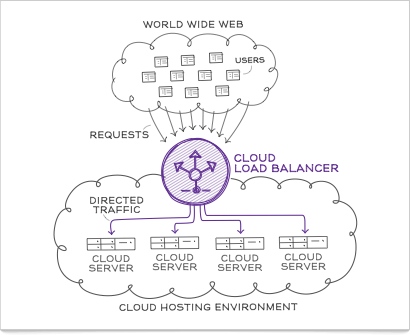
\includegraphics[width=0.50\textwidth]{img/cloud_balancer.png}
	\end{center}
	\legend{Fonte: \citeonline{rack}}
\end{figure} 

Tal conceito se torna essencial quando aplicado a computação em nuvem, uma vez que esse tipo de modelo depende necessariamente da disponibilidade e do tempo de resposta. Isto, acrescido dos conceitos essenciais para Computação em Nuvem apresentam o balanceamento de carga como um problema que requer atenção no contexto de computação em nuvem \cite{sran2013comparative}. Assim, a distribuição de carga através da nuvem impacta diretamente no desempenho geral do sistema. 

Identificar os desafios encontrados no balanceamento de carga em sistemas de nuvem é um dos caminhos para entender quais características um algoritmo de balanceamento de carga deve funcionar de modo satisfatório. Segundo \citeonline{surveycloud:2012}, pode-se citar os seguintes tópicos: 

\begin{itemize}
	\item distribuição esparsa dos nós da nuvem: consiste em um desafio visto que criar um algoritmo capaz de funcionar em arquiteturas esparsas e altamente distribuídas torna-se difícil, visto que é preciso levar em consideração a distancia entre os nós e consequentemente, adequar o algoritmo a atrasos; 
	
	\item armazenamento/replicação: a replicação de dados entre os nós pode resultar em maior custo, uma vez que mais capacidade de armazenamento é requerida;
	
	\item complexidade do algortimo: é preferível que algoritmos de balanceamento não sejam tão complexos em termos de implementação, pois isto pode resultar em requisições maiores de informação aumentando o tempo de resposta, o que diminui a eficiência; 
	
	\item ponto de falha: a coleta de dados acerca das informações sobre nós diferentes deve ser projetada com o intuito de evitar erros no algoritmo. Geralmente algoritmos centralizados tendem a ser mais eficientes para certos tipos de arquiteturas, mas costumam falhar em outras. Algoritmos distribuídos, por sua vez, possuem uma abordagem melhor, mas mais complexa.
\end{itemize}

Os algoritmos de balanceamento de carga podem ser divididos, de forma generalizada, em estáticos - associa cargas com base na habilidade do nó de processar tarefas, sem levar em consideração mudanças em tempo real - e dinâmicos - considera diferentes aspectos dos nós, incluindo capacidade e largura de banda \cite{surveycloud:2012}. 

É importante ressaltar que o balanceamento preferivelmente deve ser feito de forma dinâmica, visto que o comportamento da nuvem pode variar e a infraestrutura geralmente é composta de \textit{hardwares} distintos. Além disto, a distribuição de carga busca melhorar a eficiência de sistemas distribuídos considerando questões que ainda apresentam-se como desafios na área de computação em nuvem, tais como gerenciamento eficiente de tráfico, gerenciamento de energia e alocação dinâmica de recursos\cite{zhang2010cloud}. Tendo isto em vista, existem critérios que devem ser considerados na definição das métricas que quantificam a efetividade de algoritmos de balanceamento. Ainda segundo \citeonline{surveycloud:2012}, podemos citar os seguintes critérios: 

\begin{enumerate}
	\item taxa de transferência - relacionado ao número de tarefas completadas; 
	\item custo associado ao algoritmo de balanceamento; 
	\item tolerância a falhas;
	\item tempo de resposta; 
	\item escalabilidade e flexibilidade na capacidade de distribuição das cargas de acordo com a demanda, bem como se adequar rapidamente às demandas; 
	\item utilização de recursos;
	\item desempenho do sistema. 	
\end{enumerate}


Pode-se considerar que os objetivos do balanceamento de carga são, de maneira geral, melhorar o desempenho do sistema a um custo mais baixo; garantir a escalabilidade e flexibilidade, de forma que o algoritmo se adapte facilmente à possíveis mudanças no sistema e, por fim, garantir que a prioridade (caso haja) seja respeitada\cite{kaur2012load}. 

Diversos algoritmos de balanceamento foram propostos, com abordagens distintas, mas sempre tentando atender da melhor forma possível os objetivos de balanceamento de carga. Dentre eles pode-se citar o \textit{Round Robin} \cite{soni2014novel}, \textit{Biased Random Sampling} \cite{randles2010comparative1}, \textit{Active Clustering} \cite{randles2010comparative1}, \textit{Ant Colony}\cite{nishant2012load} e \textit{Honeybee Foraging Behavior} \cite{randles2010comparative1}.  

\newpage
% ---
\section{Redes Nerais Artificiais}\label{sec:rna}
% ---

Técnicas de reconhecimento de padrões tem por objetivo aprender funções de decisão que separam um conjunto de dados em agrupamentos de amostras (\textit{clusters}) que compartilham propriedades similares\cite{Duda:00}. Tal processo de aprendizado de funções de decisão podem ser geralmente associados a três abordagens: (i) supervisionada, na qual, a princípio, se conhece informações sobre todo o conjunto de treinamento; (ii) semi-supervisionado, no qual parte das informações sobre o conjunto de treinamento é conhecido e (iii) não-supervisionado, no qual não se tem informações prévias a respeito das amostras do conjunto de treinamento. 

Técnicas supervisionadas são conhecidas por apresentarem melhores taxas de acurácia, uma vez que a quantidade de informações disponíveis acerca das amostras de treinamento permite que tais técnicas aprendam a classificar de maneira específica determinadas propriedades, bem como permite a construção de estruturas mais complexas de aprendizagem de forma a aprimorar a qualidade do processo de treinamento.

O estado da arte neste campo tem como referência técnicas como Máquinas de Vetores Suporte (\textit{Support Vector Machines – SVM}), proposta por \citeonline{cortes1995support}, Redes Neurais (\textit{Neural Networks}), amplamente discutidas por Haykin (2007), classificadores Bayesianos e os amplamente conhecidos k-médias ( \textit{k-nearest neighbours – k-NN}), dentre outros\cite{Duda:00}. 

Dentro do contexto de reconhecimento e classificação de padrões, as Redes Neurais Artificiais tem sido amplamente estudadas em diferentes contextos de aplicações. Há, atualmente, diversos tipos de configurações de arquiteturas destas redes. De forma geral, sua arquitetura é formada por camadas de neurônios, sendo a configuração mais trivial composta por uma camada de entrada (\textit{input layer}), uma ou mais camadas escondidas (\textit{hidden layer}) e uma camada de saída (\textit{output layer}). Cada neurônio em sua respectiva camada recebe um estímulo que é processado pelo neurônio e propagado à camada seguinte, como representado na figura 3. 
\begin{figure}[ht!]
	\caption{Estrutura de uma ANN}
	\label{fig:ann-arq}
	\begin{center}
		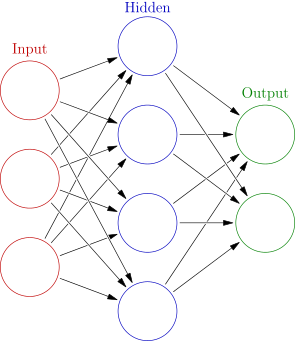
\includegraphics[scale=0.48]{img/ann-arq.png}
	\end{center}
	\legend{Fonte: \citeonline{wiki}}
\end{figure}

As Redes Neurais Artificiais ou \textit{Artificial Neural Networks - ANN} são compostas por elementos chamados neurônios, os quais, segundo \citeonline[p.~11]{Haykin2ndnew}, são unidades de processamento que ao receber um valor de entrada (ou \textit{input}) são responsáveis por processá-lo e propagar o sinal para a próxima camada. Este processamento pode ocorrer, basicamente, de três formas diferentes: 
\begin{itemize}[noitemsep]
	\item multiplicação da entrada por um peso; 
	\item o neurônio funciona tal qual um somador, ou combinador linear de suas entradas;
	\item o sinal de entrada é parâmetro de uma função de ativação responsável por limitar a amplitude do sinal de saída, como ocorre em uma sigmoide, por exemplo.
\end{itemize}

Dentro deste contexto, há atualmente uma diversidade muito grande de arquiteturas nas quais é possível organizar essas pequenas unidades. O poder de aprendizado das redes neurais permite efetuar desde tarefas mais simples, até atuar em complexos sistemas de aprendizado e classificação, como por exemplo, no reconhecimento de imagens e voz - basta ver exemplos como os das Redes Neurais Recorrentes (\textit{Recurrent Neural Networks - RNN})\cite{rnn} ou Redes Neurais de Convolução (\textit{Convolutional Neural Networks - CNN}). Dentre as aplicações de ANNs, podemos citar o uso no controle, classificação, previsão, como filtros para extrair informações, dentre outras. 

No entanto, nem todos os problemas exigem arquiteturas tão complexas. Segundo \citeonline[p.~21-23]{Haykin2ndnew}, há três tipos fundamentais de estruturas: \textit{Single Layer Feedfoward Networks} (Redes Neurais de Camadas Únicas), \textit{Multilayer Feedfoward Networks} (Redes com Múltiplas Camadas) e \textit{Recurrent Networks} (Redes Neurais Recorretes).

\begin{figure}[ht!]
	\caption{Fluxo de aprendizado de uma rede neural}
	\label{fig:annfluxo}
	\begin{center}
		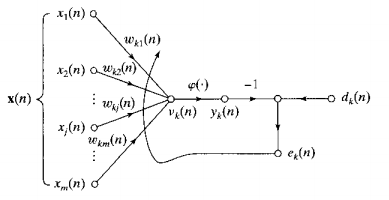
\includegraphics[scale=0.8]{img/annflowlearning.png}
	\end{center}
	\legend{Fonte: \citeonline[p.~52]{Haykin2ndnew}}
\end{figure}

É importante ressaltar que a quantidade de camadas em uma rede impacta diretamente no desempenho em relação ao processamento e na velocidade de aprendizado. Além disso, a escolha de implementações de arquiteturas que atendam à um problema específico ou sejam demasiadamente especializadas não é recomendado pois pode tornar a arquitetura ineficiente na resolução de problemas diferentes daqueles na qual foi treinada. 

\subsection{Perceptron}

Perceptrons de única camada são uma alternativa simples de implementação de rede neural para identificar dados que são linearmente separáveis. O conceito aplicado é de uma rede que recebe vetores de características que treinam o Perceptron para identificar padrões e classificar amostras. Um neurônio também forma uma base de um filtro adaptativo, que pode ser aplicado em um sistema dinâmico. De forma geral, a Figura \ref{fig:annfluxo} representa a propagação de sinal por um modelo adaptativo. No caso de um Perceptron, a propagação de sinal é feita por meio de uma função não-linear. A representação do fluxo de sinal de um Perceptron, ilustrado na Figura \ref{fig:perceptron}, denota exatamente este fluxo de processamento. 
	
\begin{figure}[ht!]
	\caption{Fluxo de sinal em um Perceptron}
	\label{fig:perceptron}
	\begin{center}
		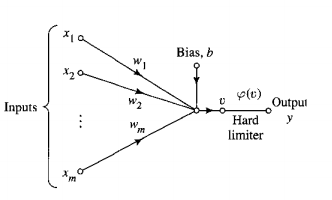
\includegraphics[scale=0.8]{img/perceptron.png}
	\end{center}
	\legend{Fonte: \citeonline[p.~136]{Haykin2ndnew}}
\end{figure}	

O Perceptron tem em seu modelo um fluxo (representado na figura \ref{fig:perceptron}) no qual os pesos $w_1, w_2, ... , w_m$ são sinapses do Perceptron, correspondentes à cada uma de suas respectivas entradas, denotadas por $x_1, x_2, ... , x_m$. Uma \textit{bias} pode ser aplicada externamente, denotada por $b$. O nó $ v $ recebe a propagação do sinal e, a partir da aplicação de uma função propaga a saída $y$ (\textit{Output}). A partir do modelo, pode-se inferir que o limitador da camada de entrada, ou local de indução dos neurônios é denotado pela equação \ref{eq:funcperceptron}.  

\begin{equation}
v = \sum_{i=1}^{m} ({w_i} \times {x_i} + b)
\label{eq:funcperceptron}
\end{equation}

O objetivo de um Perceptron, de forma geral, é classificar corretamente a entrada, ou seja, $x$ em uma de duas classes, $C_1$ ou $C_2$. Neste contexto, a regra de decisão associa o ponto representado pelo vetor $x$ em uma das classes, dada sua saída. Os pesos em $w$ podem ser ajustados a cada iteração e, para isso, usa-se uma função de ajuste, seja por correção de erro, seja por regras de convergência \citeonline{Haykin2ndnew}. Nesse caso, um dos algoritmos que pode ser seguido está representado a seguir:
\begin{enumerate}
	\item \textit{inicialização de paramêtros}: inicialização do vetor de pesos (lembrando que a atualização é feita em $n$ \textit{steps} ou iterações);
	\item \textit{ativação}: em cada \textit{step}, receber a entrada (ou \textit{input}) e ativar o Perceptron;
	\item \textit{computar a saída}: resposta do perceptron $y(n)$, ou seja, a saída da função de ativação;
	\item \textit{ajuste}: ajuste dos pesos de $w$ 
	\item \textit{continuação}: repetição do processo	 
\end{enumerate}

\subsection{\textit{ANNs} com Múltiplas Camadas}



Como variação do Perceptron tem-se uma rede de múltiplas camadas, chamada Perceptron Multicamada (PMC), que são constituídas de um conjunto de neurônios sensoriais que formam uma camada de entrada, uma ou mais camadas ocultas de nós computacionais e uma camada de saída, também com nós computacionais. O sinal de entrada, recebido pela camada de entrada, é propagado para a próxima camada, repetindo esse processo até a camada de saída\citeonline[p.~98]{Haykin98p93}. 

Cada neurônio possui uma função de ativação, geralmente não-linear. A não linearidade dessa função é importante para a saída da rede, visto que permite que valores de classificação não binária sejam atribuídos, o que permite que haja classificação de duas ou mais classes. A camada escondida capacitam a rede a aprender tarefas complexas extraindo progressivamente as características mais significativas. A Figura \ref{fig:pmc} apresenta a estrutura generalizada de um Perceptron Multicamadas. 

\begin{figure}[ht!]
	\caption{\label{fig:pmc}Estrutura de um Perceptron Multicamada}
	\begin{center}
		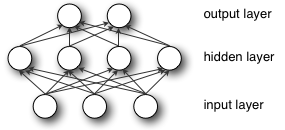
\includegraphics[width=0.5\textwidth]{img/mlp.png}
	\end{center}
	\legend{Fonte: \citeonline{mlp}}
\end{figure}

Redes Neurais de Base Radial (\textit{Radial Basis Function - RBF}) é uma rede neural semelhante ao PMC constituída por no mínimo três camadas, sendo uma de entrada, uma escondida e uma de saída. Nesta rede, a camada de entrada recebe um vetor de características ao qual é aplicada uma transformação não-linear na camada escondida. A Figura \ref{fig:rbf2} apresenta a estrutura de uma RBF genérica. 

\begin{figure}[htb]
	\caption{\label{fig:rbf2}Estrutura de uma Rede Neural com função de Base Radial}
	\begin{center}
		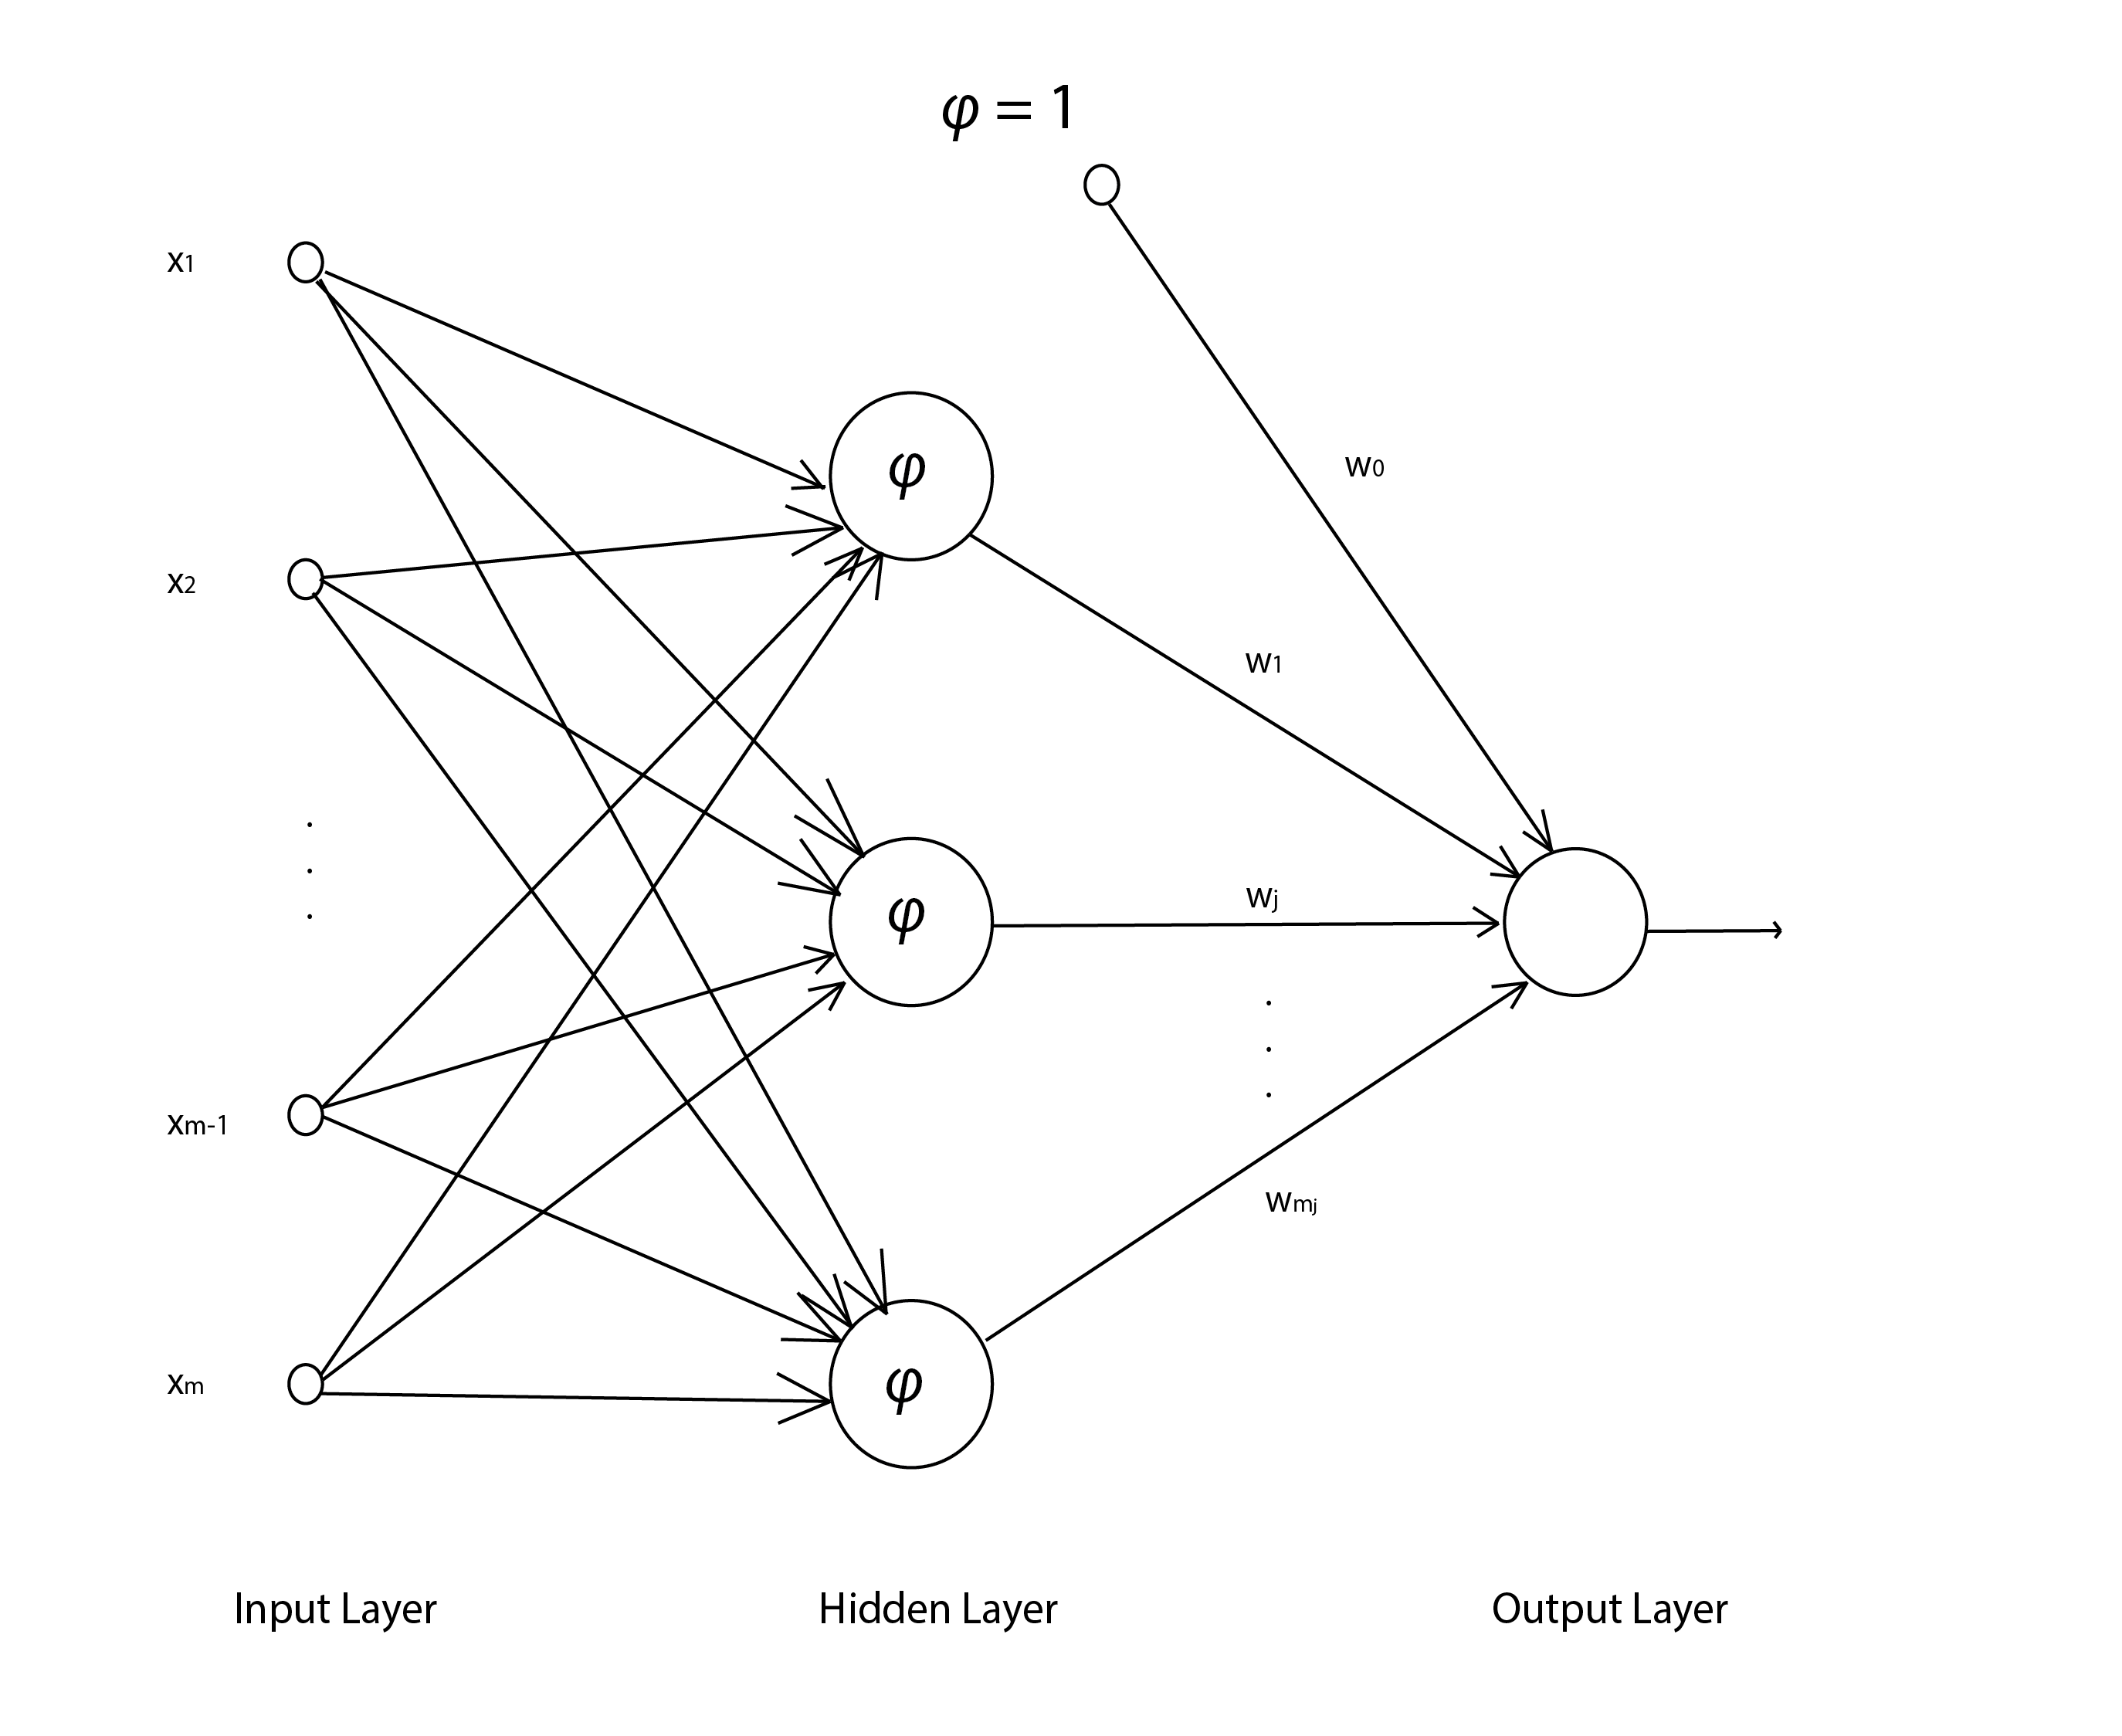
\includegraphics[width=0.60\textwidth]{img/rbf2.png}
	\end{center}
	\legend{Fonte: Baseado em \citeonline[p.~278]{Haykin2ndnew}}
\end{figure}

O diferencial da RBF para o PCM é, além da estrutura, a função de ativação aplicada para aprender as características mais relevantes. Neste caso, a função de ativação mais empregada é a Gaussiana, por sua formulação simples. 

Existem outros tipos de redes,tais quais as Redes Neurais Probabilística (\textit{Probabilistic Neural Network - PNN})\cite{specht1990probabilistic}, que funcionam de maneira semelhante a uma RBF. Sua camada escondida, no entanto, e dividida em duas partes: uma camada de padrões e uma camada de somatório. A Figura 6 apresenta a estrutura generalizada de uma PNN. A primeira tem por objetivo calcular a probabilidade de um determinado vetor de característica \textit{y} pertencer à uma classe \textit{x}. A segunda camada, por sua vez, realiza um somatório dessas probabilidades. Na camada de saída, os dados recebidos da camada anterior são utilizados para classificar as amostras, atribuindo a \textit{y} o rótulo correspondente ao neurônio com maior probabilidade.

% ----------------------------------------------------------